% !TEX root = main.tex

We now outline the core algorithm of AMIE and its implementation.
We follow the description in \cite{amie} and extend it with further explanations and details.

\subsection{Algorithm}
\label{subsec:algorithm}

%Only overview in this point
\paragraph{Algorithm} Algorithm~\ref{rm} shows our approach to mine rules. It takes as input a KB $\mathcal{K}$,
a threshold $minHC$ on the head coverage of the mined rules, a maximum rule length $maxLen$
and a threshold $minConf$ on the confidence. We discuss the choice of parameter values later in this section.
The algorithm maintains a queue of rules (line~1), which initially contains all possible head atoms, that is, all rules of size 1.
It then iteratively dequeues a rule from this queue.
If the rule meets certain criteria (line~6), it is pushed to the output.
If the rule does not exceed the maximum number of atoms $maxLen$ (line~9), it goes through a refinement process (described below) which
expands the rule (the parent) to produce a set of new rules (the children). These new rules,
if neither duplicates nor pruned by the head coverage threshold (line~12),
are also pushed into the queue.
This process is repeated until the queue is empty.
In the following, we will see in more detail the different phases of the algorithm.

\begin{algorithm}
\caption{Rule Mining}
\label{rm}
\begin{algorithmic}[1]
\Function{AMIE}{KB $\mathcal{K}$, $minHC$, $maxLen$, $minConf$}
    \State $q = [r_1(x,y), r_2(x,y) \dots r_m(x,y)] $
    \State $out = \langle \rangle$
	\While{$\neg q$\emph{.isEmpty}()}
	  \State $r = q.$\emph{dequeue}()
	  \If{$AcceptedForOutput(r, out, minConf)$}
	      \State $out.$\emph{add}$(r)$
	  \EndIf

	  \If{$length(r) < maxLen$}
	    \State $R(r) = Refine(r)$
	    \ForAll{rules $r_c \in R(r)$}
		    \If{$hc(r_c) \ge minHC$ \& $r_c \notin q$}
			\State $q.$\emph{enqueue}$(r_c)$
		    \EndIf
	    \EndFor

	  \EndIf

	\EndWhile
    \State \Return $out$
\EndFunction
\end{algorithmic}
\end{algorithm}

\paragraph{Refinement}\label{subsubsec:refinement}
One of the major challenges of rule mining is to find an efficient way to explore the search space.
The naive algorithm of enumerating all possible combinations of conjunctions of atoms is infeasible for large KBs.
Hence, we explore the search space by iteratively extending rules using a set of \emph{mining operators} (line~10 of Alg.~\ref{rm}).
We see a rule as a sequence of atoms. The first atom is the head atom and the others are the body atoms.
In the process of traversing the search space, we can extend a rule by using one of the following operators:
\begin{enumerate}
\item \textbf{Add Dangling Atom ($\mathcal{O}_D$})\\
This operator adds a new atom to a rule. The new atom uses a fresh variable for one of its two arguments. The other argument is a variable
that is shared with the rule, i.e., it occurs in some other atom of the rule.
\item \textbf{Add Instantiated Atom ($\mathcal{O}_I$})\\
This operator adds a new atom to a rule that uses an entity for one argument and shares the other argument (variable) with the rule.
\item \textbf{Add Closing Atom ($\mathcal{O}_C$})\\
This operator adds a new atom to a rule so that both of its arguments are shared with the rule.
\end{enumerate}
Note that all above operators create connected rules.
By repeated application of these operators, we can generate the entire space of rules as defined in Section~\ref{sec:preliminaries}.
The operators generate even more rules than those that we are interested in, because they also produce rules that are not closed.
An alternative set of operators could consist of $\mathcal{O}_D$ and an operator for instantiation.
But these operators would not be monotonic, in the sense that an atom generated by one operator can be modified in the next step by the other operator.
Therefore, we chose the above 3 operators as a canonic set. We will describe in Section \ref{subsec:countqueries} how these operators are executed on the KB.

\begin{algorithm}
\caption{Decide whether to output a rule}
\label{pfo}
\begin{algorithmic}[1]
\Function{AcceptedForOutput}{rule $r$, $out$, $minConf$}
    \If{$r$ is not closed $\vee\; conf_{pca}(r) < minConf$}
      \State \Return $false$
    \EndIf
    \State $parents = parentsOfRule(r, out)$
    \ForAll{$r_p \in parents$}
      \If{$conf_{pca}(r) \le conf_{pca}(r_p)$}
	\State \Return $false$
      \EndIf
    \EndFor
    \State \Return $true$
\EndFunction
\end{algorithmic}
\end{algorithm}

\paragraph{When to Output}\label{subsubsec:whenToOutput}
Not every rule that the mining algorithm dequeues is output. This is because some rules may not be closed, or may not be better than rules that have already been output. Algorithm~\ref{pfo} explains how we decide if a rule should be output or not once it has been dequeued.
The algorithm first checks if the rule is of the form described in Section~\ref{sec:preliminaries} (i.e., closed and connected).
The refinement operators used by AMIE (see Section~\ref{subsubsec:refinement}) always produce connected rules.
So, at this point, the algorithm only checks if the rule is closed. Then, the algorithm calculates
the confidence of the rule and performs a quality check. The rule should have a confidence value that (i) passes the confidence threshold (line~1)
and (ii) improves over the confidence of all its parents (line~7).
The latter condition implies that the refinements of a rule ($B_1 \wedge ... \wedge B_n \wedge B_{n+1} \Rightarrow H$) must
bring some confidence gain with respect to the parent rule
($B_1 \wedge ... \wedge B_n \Rightarrow H$). Since support and head coverage are monotonic metrics,
we know that the child rule will never have a higher score than its parent rule.
If the child rule has also lower confidence, then its quality is worse in all aspects than the parent rule. Hence, there is no reason to output it.

A rule can have several parents. For example, the rule $actedIn(x,y) \wedge directed(x,y) \Rightarrow created(x,y)$
can be derived by either adding $directed(x,y)$ to  $actedIn(x,y) \Rightarrow created(x,y)$ or by adding $actedIn(x,y)$ to
$directed(x,y) \Rightarrow created(x,y)$. AMIE requires a confidence gain over all parents of a rule.

Note that the decisions made at this point affect only the output. They do not influence the refinement process. i.e., a rule with low confidence can still be refined to obtain new rules.
This is because confidence is a non-monotonic measure, i.e., we might get good rules with further refinement of bad rules.


\paragraph{Parameters and Pruning}
If executed naively, Algorithm~\ref{rm} will have prohibitively high runtimes.
The instantiation operator $\mathcal{O}_I$, in particular, generates atoms in the order of $|\mathcal{R}| \times |\mathcal{E}|$.
For this reason the algorithm defines some parameters that determine when to stop with the exploration of the space.
These are the minimal head coverage $minHC$, the maximal length $maxLen$ and the minimal confidence $minConf$.
% The algorithm traverses the search space and enumerate all rules that fulfil the constraints
% of a minimal head coverage $minHC$, a minimal confidence $minConf$, and a maximal length of $maxLen$.
%Thus, these parameters define when the algorithm shall stop with the exploration of the space.
Choosing larger thresholds on head coverage, and choosing a shorter maximum rule length will make the algorithm stop earlier
and output fewer rules. Relaxing the values will make the algorithm output the very same rules as before,
and find also rules with a smaller head coverage or a larger number of atoms.
Thus, these parameters define a trade-off between the runtime and the number of rules.

Interestingly, a larger number of rules is not necessarily a good thing.
For instance, a rule that covers only 1\% or less of the instances of a relation is probably not interesting. It simply lacks statistical significance. Assuming that a user is not interested in such spurious rules, we set $minHC=0.01$ by default.
% \comment{chris}{Additionally, we show in our experiments that rules with more than 3 atoms tend to be very convoluted and not insightful. Hence, we set $maxLen=3$.}

Additionally, we show in our experiments that rules with more than 3 atoms tend to be very convoluted and not insightful. Hence, we set $maxLen=3$ by default.

%Additionally, our experience with web-extracted KBs suggests that a rule length of 3 offers a good trade-off
%between mining speed and expressivity of rules. Hence, we set $maxLen=3$.

Likewise, rules with low confidence will not be of much use to the application. For example, a rule with confidence 10\% will make correct predictions in only one out of
ten cases. Assuming that a user is not interested in such kind of rules, we set $minConf=0.1$ by default.

%Notice also that Algorithm~\ref{rm} does not use confidence for pruning. This implies that the confidence
%threshold does not have a significant impact in the runtime as head coverage and maximum length.
% Likewise, a rule that covers only 1\% or less of the instances of a relation is probably not interesting.
% Therefore, we set the default value $minHC=0.01$. We show in our experiments that rules with more
% than 3 atoms tend to be very convoluted and not insightful.
% Hence, we set $maxLen=3$.

That being said, if the user is interested in less confident, more complex, or less supported rules,
she can change these thresholds. However, we believe that there is no good reason to deviate from the default values.
In particular, relaxing these values will not output better rules. This makes AMIE a system that can be run off the shelf,
without the need for parameter tuning.

% \ignore {
% \paragraph{Pruning}
% If executed naively, Algorithm~\ref{rm} will have prohibitively high runtimes.
% The instantiation operator $\mathcal{O}_I$, in particular, generates atoms in the order of $|\mathcal{R}| \times |\mathcal{E}|$.
% We first observe that we are usually not interested in rules that cover only very few facts of the head relation.
% Rules that cover, for example, less than 1\% of the facts of the head relation can safely be assumed to be marginal.
% Therefore, we choose $minHC=0.01$ as a lower bound for the head coverage. We observe that head coverage decreases monotonically as we add more atoms.
% This allows for safely discarding any rule that trespasses the threshold (line~12 of Alg.~\ref{rm}).
% Recall from Section~\ref{subsec:statSignificance} that support and head coverage are defined even for rules that are not yet closed, allowing for early pruning.
% }
\paragraph{Duplicate Elimination} \label{subsec:duplicateElimination}
As mentioned in Section~\ref{subsubsec:whenToOutput} a rule can be derived in multiple ways.
For example, the rule $actedIn(x,y) \wedge directed(x,y) \Rightarrow created(x,y)$ can result from the application
of the operator $\mathcal{O}_C$ to both $actedIn(x,y) \Rightarrow created(x,y)$ and $directed(x,y) \Rightarrow created(x,y)$.
For this reason, AMIE checks for the existence of duplicate rules (line~12) in order to avoid queuing the same rule multiple times.
While checking two rules for equality is expensive (it is a graph isomorphism verification task),
we observe that two rules can only be equal if they have the same head relation, the same number of atoms and
the same head coverage (or support). This reduces drastically the set of rules that have to be checked and therefore
the time invested in this task.


\paragraph{Multithreading}
To speed up the process, our implementation parallelizes Algorithm~\ref{rm}, that is, the main loop (lines~4 to~17) runs in multiple threads.
This is achieved by synchronizing the access to the centralized queue from which the threads dequeue and enqueue and the access to the output.
%In addition, when AMIE uses multiple threads, there is a need for an additional duplicate-elimination check at line~6 of Alg.~\ref{rm}. \comment{Fabian}{Can we avoid the discussion of dup elimination in the output here? I am afraid it might raise more questions than it anwers...}

\ignore{
\comment{Chris}{@Luis: why don't you use barriers here? I.e., all threads wait until there is no rule length n in the queue before moving to the rules with length n+1. For rules with 3 atoms in the body
you will only have 2 synchronization points.}
Recall that our algorithm performs a breadth-first-search.
This means that in a fully sequential execution, all the rules of size $n-1$ are always queued before all the rules of size $n$.
It follows that, by the time we check the duplicates of a rule of size $n$ to enqueue it (line~12 in Algorithm~\ref{rm}),
no rule of size $n$ has still been dequeued. In other words, if a rule is the duplicate
of another rule already derived, the original rule must be in the queue. This property guarantees no duplicates at output time.

However, this does not hold in a multi-threading environment.
To see this, imagine that rules
$R_n$ and $R'_n$ are both in the queue at timestamp $t_0$ and both can refined into rule $R_{n+1}$
by means of the mining operator $o$.
Moreover, consider two threads $T_1$ and $T_2$ and the sequence of events depicted in Table~\ref{tab:duplicates}.

\begin{table}
\centering
 \begin{tabular}{c|l|l}
  Timestamp & $T_1$ & $T_2$\\  \hline
  $t_1$ & $R_n = q.dequeue()$	&  \\
  $t_2$ & & $R'_n = q.dequeue()$ \\
  $t_3$ & $R_{n+1} = o(R_n)$  & \\
  $t_4$ & $q.enqueue(R_{n+1})$  & \\
  $t_5$ & $R_{n+1} = q.dequeue()$ & \\
  $t_6$ & & $R_{n+1} = o(R'_n)$ \\
  $t_7$ & & $q.enqueue(R_{n+1})$ \\
\end{tabular}
\caption{An execution scenario that could lead to duplicate rules in the output.}\label{tab:duplicates}
\end{table}

In this example, we enqueue the rule $R_{n+1}$ twice, at timestamps $t_4$ and $t_7$.
Since $T_1$ dequeues $R_{n+1}$ before $T_2$ also finds it,
we cannot know that the rule was already output before.
Since duplicate verification
can be performed very efficiently, we show that the time invested in this additional step does not
outweigh the benefit of using multiple threads.
}


\subsection{Count Projection Queries}
\label{subsec:countqueries}

AMIE tries to expand a given rule by applying all mining operators defined in the last section (one each time).
We now explain how the operators are implemented and executed on a KB.

\paragraph{Count Projection Queries}
%Each operator expects as input a variable that the new atom shall share with the existing rule.
Assume that AMIE needs to add the atom $r(x,y)$ to a rule.
For efficiency reasons, we do not blindly try all possible relations in the place of $r$. Instead, we first
find all relations that lead to a new rule that passes the head-coverage threshold.
In other words, we first fire a \emph{count projection query} of the form

\indented{
SELECT $\bm{r}$, COUNT($H$)\\
WHERE $H \wedge B_1 \wedge ... \wedge B_{n-1}\; \wedge\; \bm{r}(\bm{X},\bm{Y})$\\
SUCH THAT COUNT($H$)$\geq k$
}

\noindent where $k := minHC \times size(H)$ (see Section~\ref{par:headCoverage}) is the translation of the
head coverage threshold into an absolute support threshold and the expression COUNT($\cdot$)
has COUNT(DISTINCT $\cdot$) semantics (also for the rest of this section).
$\bm{X}$ and $\bm{Y}$ represent variables that are either fresh or already present in the rule.
%\comment{Luis}{About the meta-variables, the text originally said ``that can be either variables or constants, depending on the type of atoms that the operator generates". I changed because in principle we never add atoms where one of the arguments is a constant, because we first find the relationand then the constants for the arguments.}
% Fabian: fine...
The results for $\bm{r}$ are the relations that, once bound in the query,
ensure that the head coverage of the rule $B_1 \; \wedge ... \wedge B_{n-1} \;\wedge\; \bm{r}(\bm{X},\bm{Y}) \Rightarrow H$ is greater
or equal than $minHC$.
Notice also that for each value of $\bm{r}$, the expression COUNT($H$) gives us the support of the new rule.
We now discuss the instantiation of this query for all three operators.

\paragraph{Dangling Atom Operator}
% When we apply the $\mathcal{O}_I$ operator, at least one of this meta-variables binds to a constant.
As an example, assume that Algorithm~\ref{rm} dequeues the following intermediate non-closed rule for further specialization:

\indented{
\emph{marriedTo}$(x,z) \Rightarrow $ \emph{livesIn}$(x,y)$
}

\noindent
The application of the operator $\mathcal{O_D}$ will fire queries of the form:

\indented{
SELECT $\bm{r}$, COUNT($livesIn(x,y)$) WHERE  \\
$livesIn(x,y) \; \wedge \; marriedTo(x,z) \wedge \bm{r}(\bm{X}, \bm{Y})$\\
SUCH THAT COUNT($livesIn(x,y)$)$\ge k$
}

\noindent with
\indented{
$\bm{r}(\bm{X}, \bm{Y}) \in \{\bm{r}(x,w), \bm{r}(z,w), \bm{r}(w,x), \bm{r}(w,z) \}$
}

\noindent That is, $\bm{r}(\bm{X}, \bm{Y})$ binds to each possible join combination of a new dangling atom,
where $w$ is an arbitrary fresh variable. For intermediate rules, dangling atoms are joined on the non-closed variables;
$z$ and $y$ in this example.
If the rule is closed, dangling atoms are joined on all the variables appearing in the rule.

\paragraph{Closed Atom Operator} The $\mathcal{O_C}$ operator works in the same fashion. In our example, the atom $\bm{r}(\bm{X}, \bm{Y})$
can take values in $\{ \bm{r}(z,y), \bm{r}(y,z) \}$. The method will produce new atoms so that all open variables are closed. In this example, the method produces the minimum number
of specializations required to close the variables $y$ and $z$. If there is only one closed variable, the method will produce atoms between
the open variable and all the other variables. If the rule is already closed, the operator tries with
all possible pairs of variables in the rule.

\paragraph{Instantiated Atom Operator} The operator $\mathcal{O_I}$ is implemented in two steps.
We first apply the operator $\mathcal{O_D}$ to produce a set of intermediate rules
with a new dangling atom and a new fresh variable.
Then for each rule, we fire a count-projection query on the fresh variable.
This step provides bindings for one of the arguments of the relation.
For instance, the application of the $\mathcal{O_I}$ operator to our example
rule

\indented{
\emph{marriedTo}$(x,z) \Rightarrow $ \emph{livesIn}$(x,y)$
}

\noindent will first add all possible dangling atoms to the rule. Let us consider one group of such atoms, e.g., those of the form
$\bm{r}(x,w)$. Then for each
value of $\bm{r}$ that keeps the rule above the head coverage threshold $minHC$, the algorithm tries to find the best bindings for
$w$. For example, imagine we bind $\bm{r}$ to the relation $citizenOf$. The second step will fire a query of the form:

\indented{
SELECT $\bm{w}$, COUNT($livesIn(x,y)$) WHERE \\
$livesIn(x,y) \wedge marriedTo(x,z) \wedge citizenOf(x,\bm{w})$ \\
SUCH THAT COUNT($livesIn(x,y)$)$\ge k$
}

\noindent Each binding of $\bm{w}$ forms a new rule that will be enqueued and later evaluated for output.

Count-projection queries allow us to choose the relationships and entities for the operators
in such a way that the head coverage for the new rules is above $minHC$.
We discuss how to implement count projection queries efficiently in Section~\ref{subsec:implementation}.

\subsection{Query Implementation Details}
\label{subsec:implementation}

\paragraph{In-Memory Database} We have shown \cite{amie} that count projection queries translate into very inefficient queries in both SPARQL and SQL. Therefore, we have implemented an in-memory database that is specifically geared towards this type of queries.
Our implementation indexes the facts aggressively with one index for each permutation of
the columns subject (\texttt{S}), relation (\texttt{R}), and object (\texttt{O}). This means that there are six indexes, namely \texttt{SRO}, \texttt{SOR}, \texttt{RSO}, \texttt{ROS}, \texttt{OSR} and \texttt{ORS}. We call them \emph{fact indexes}.
Each fact index is a hash table, which maps elements of the first column to a nested hash table. This nested hash table maps elements of the second column to a set of elements of the third column. For example, the index \texttt{ORS} has as keys the objects of all triples in the KB. It maps each object $o$ to a hash table. This hash table has as keys all possible relations of the KB. It maps each relation $r$ to a set of subjects $\{s_1,...,s_n\}$, such that $r(s_i, o)$ for $i=1...n$.
Fact indexes allow us to check the existence of a triple in constant time. They also allow us to efficiently fetch the instantiations of an atom.

%where the keys are the values for the first column and the items are again hash tables. The nested hash tables map values of the second column to sets of values of the third column.
%Figure~\ref{indexes} illustrates the structure of the fact index \texttt{RSO} for a set of four facts.
%
% \begin{figure}
% %\hspace*{-5ex}
% 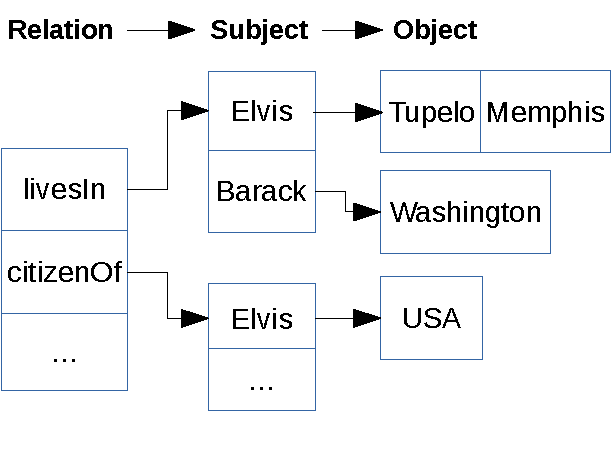
\includegraphics[width=0.5\textwidth]{figures/indexes}\
% \caption{Structure of the fact index RSO for a set of four facts}
% \label{indexes}
% \end{figure}

In addition to the fact indexes, our database relies on three \emph{aggregated indexes} \texttt{S}, \texttt{P}, \texttt{O}. These store the aggregated number of facts for each
key of the fact indexes. For example, the aggregated index \texttt{P} stores the number of triples for each relation in the KB, whereas the aggregated index \texttt{S} stores the number of triples where each entity appears as subject.

\paragraph{Size Queries} Fact indexes in combination with aggregated indexes can be used to determine the \emph{size of an atom} ($size(a,\mathcal{K})$), i.e., its number of bindings in the KB $\mathcal{K}$. For example, the size of the atom $livesIn(x,y)$ can be retrieved by a simple look-up
in the aggregated index \texttt{P}. The size of the atom $livesIn(x, USA)$ requires two
lookups in the fact index \texttt{ROS}: the first lookup to get the object values of $livesIn$ and the second
to retrieve the list of subjects for the object value $USA$.
%If an atom has size greater than zero, it means that there exists a query answer for it in the KB.
% Fabian: let's not mix existence and sizes here (even though it's trivial, I agree)...

\paragraph{Existence Queries} One of the central tasks of the in-memory database is to determine whether there exists a binding for a conjunctive query. Algorithm~\ref{exists} shows how this can be implemented.  The algorithm requires as input a conjunctive query and a KB $\mathcal{K}$.
If the query is a single atom (Line 3), we can directly verify if its size is greater than zero using
the indexes (Line 4). Otherwise, we select the atom $B_s$ with fewest instantiations using the indexes (Line 6),
and run through all of its instantiations (Lines 8 to 13). We apply such instantiations to the remaining atoms (Line 9)
and repeat this process recursively (Line 10) until we end up with a single atom. Since rules are connected query patterns, the atom $B_s$ must share at least
one variable with the remaining atoms. This means that by instantiating $B_s$, some variables in the remaining atoms
become instantiated, making the atoms more selective with every recursive step.

\begin{algorithm}
\caption{Existence Queries}
\label{exists}
\begin{algorithmic}[1]
\Function{Exists}{$B_1 \wedge ... \wedge B_n$, $\mathcal{K}$}
    \State $q := B_1 \wedge ... \wedge B_n$
    \If {$n = 1$}
      \State \Return size($B_1$, $\mathcal{K}$) $> 0$
    \Else
      \State $s := argmin_i\;\{ size(B_i, \mathcal{K}) \}$
      \State $q := q \setminus \{ B_s \} $
      \ForAll {instantiations $b_s \in B_s$}
	\State $q' := q$ instantiated with bindings from $b_s$
	  \If{Exists($q'$, $\mathcal{K}$)}
	    \State \Return true
	  \EndIf
      \EndFor
    \EndIf
    \State \Return false
\EndFunction
\end{algorithmic}
\end{algorithm}

\paragraph{Select Queries}
Algorithm~\ref{select} describes the implementation of SELECT DISTINCT queries on one projection variable for a conjunction of
atoms.
The algorithm starts finding the atom with the fewest number
of instantiations $B_s$. If the projection variable $x$ is in $B_s$ (Lines 5 to 11),
the algorithm goes through all the instantiations $\hat{x}$ of $x$, instantiates
the query accordingly and checks whether there exists a solution for the instantiated query pattern in the KB (Line 8).
If there is, the solution $\hat{x}$ is added to the result set. In contrast, if the projection variable is not in the most
restrictive atom $B_s$ (Lines 13 to 17), the algorithm iterates through the instantiations of $B_s$ and recursively selects the distinct
bindings of $x$ in the remaining atoms (Line 16).

\begin{algorithm}
\caption{Select Distinct Queries}
\label{select}
\begin{algorithmic}[1]
\Function{Select}{$\bm{x}$, $B_1 \wedge ... \wedge B_n$, $\mathcal{K}$}
    \State $q := B_1 \wedge ... \wedge B_n$
    \State $s := argmin_i\;\{ size(B_i, \mathcal{K}) \}$
    \State $result := \lbrace \rbrace$
    \If{$\bm{x} \in B_s$}
      \ForAll {instantiations $\hat{x} \in \bm{x}$}
	\State $q' := q$ instantiated with $\hat{x}$ for $\bm{x}$
	\If {Exists($q'$, $\mathcal{K}$)}
	  \State $result$.add($\hat{x}$)
	\EndIf
      \EndFor
    \Else
      \State $q := q \setminus \{ B_s\}$
      \ForAll{instantiations $b_s \in B_s$}
      	\State $q' := q$ instantiated with bindings from $b_s$
      	\State $result$.add(Select($\bm{x}$, $q'$, $\mathcal{K}$))
      \EndFor
    \EndIf
    \State \Return $result$
\EndFunction
\end{algorithmic}
\end{algorithm}

\paragraph{Count Queries} To compute the confidence of a rule $\vec{B} \Rightarrow r(x, y)$, AMIE must fire a \emph{count query} to estimate the denominator
of the confidence formula. For the PCA confidence, such queries have the form:

\indented{
SELECT COUNT($x$, $y$) WHERE $r(x, y') \wedge \vec{B}$
}

\noindent where $x$, $y$ are the variables in the head atom of the rule, $\vec{B} = B_1, \dots, B_n$ are the body atoms, and $r(x,y')$
is a variant of the head atom where the least-functional variable has been replaced by a fresh variable $y'$ (see Section~\ref{subsubsec:pcaConf}).
These queries return the number of distinct bindings of the head variables
that fulfill the pattern $r(x, y')\; \wedge\; \vec{B}$. They are used to
calculate the confidence of rules. The in-memory database first fires a SELECT query on variable $x$:

\indented{
SELECT DISTINCT $x$ WHERE $r(x, y') \wedge \vec{B}$
}

\noindent Then, for each binding of $x$, it instantiates the query and fires another select query on variable $y$, adding up the number of instantiations.


\paragraph{Count Projection Queries} Count projection queries
take the form
\indented{
SELECT $\bm{x}$, COUNT($H$) WHERE $H \wedge B_1 \wedge ... \wedge B_n$\\
SUCH THAT COUNT($H$)$\geq k$
}
These are the types of queries used to determine the relations and instances for new atoms in the refinement
phase of AMIE. Algorithm \ref{algi} shows how we answer these queries. The algorithm takes as input a selection variable $\bm{x}$, a projection atom $H:=R(\bm{X},\bm{Y})$, remaining atoms $B_1, ... B_n$, the threshold $k$,
and a KB $\mathcal{K}$.
The algorithm returns a hash table with each instantiation of the selection variable
$\bm{x}$ as key and the number of distinct bindings of the projection atom $H$ as value.
%\comment{Fabian}{I added the threshold k to this algorithm, to disentangle the roles of the rule mining and the in-memory database}
%The algorithm does not consider the threshold condition (SUCH THAT), because this condition is actually enforced by the AMIE algorithm and not the in-memory database.

We first check whether $\bm{x}$ appears in the projection atom (Line 3).
If that is the case (Lines 4 to 10), we run through all instantiations of the projection atom, instantiate the query accordingly (Line 6), and check for existence (Line 7).
Each existing instantiation increases the counter for the respective value of the selection variable $\bm{x}$ (Line 8).
If the selection variable does not appear in the projection atom (Lines 12 to 18),
we iterate through all instantiations of the projection atom.
We instantiate the query accordingly, and fire a SELECT DISTINCT query for $\bm{x}$ (Line 14).
We then increase the counter for each value of $\bm{x}$ (Line 16).

\begin{algorithm}
\caption{Count Projection Queries}
\label{algi}
\begin{algorithmic}[1]
\Function{SELECT}{$\bm{x}$, $R(X,Y) \wedge B_1 \wedge ... \wedge B_n$, $k$, $\mathcal{K}$}
    \State $map = \{\}$
    \State $q=B_1 \wedge ... \wedge B_n$
    \If {$\bm{x} \in \{R,X,Y\}$}
	  \ForAll{instantiations $r(x,y) \in R(\bm{X}, \bm{Y})$}
	    \State $q' :=q$, replace $R$ by $r$, $X$ by $x$, $Y$ by $y$
	    \If{Exists($q'$, $\mathcal{K}$)}
		\State $map[x]++$
	    \EndIf
	  \EndFor
	\Else
	  \ForAll{instantiations $r(x,y) \in R(\bm{X},\bm{Y})$}
	    \State $q' := q$, replace $R$ by $r$, $X$ by $x$, $Y$ by $y$
	    \State $\mathcal{X} :=$ Select($\bm{x}$, $q'$, $\mathcal{K}$)
	    \ForAll{$x \in \mathcal{X}$}
		  \State $map[x]++$
	    \EndFor
	  \EndFor
	\EndIf
	\State $map := \{ \langle x \rightarrow n\rangle \in map : n \geq k\}$
	\State \Return $map$
\EndFunction
\end{algorithmic}
\end{algorithm}

\ignore{Fabian: This part no longer makes sense when we removed the SQL queries

\paragraph{Summary}
The AMIE algorithm iteratively builds more complex rules from simpler rules by the help of three operators.
It takes advantage of monotonic measures to prune the search space efficiently and also takes care of duplicate elimination.
We have identified projection queries as the crucial type of queries for rule mining.
Since standard database systems and standard SPARQL systems provide no specifically tuned support for these queries,
we have implemented a vanilla in-memory database, which has specific support for projection queries.
Our entire implementation is in Java. The code can be downloaded from our Web site\footnote{\url{http://mpi-inf.mpg.de/departments/ontologies/projects/amie}}.
}

%%% Uncomment this to return to the version with SQL queries.
%
% \ignore{
%
% %%%%%%%%%%%%%%%%%%%%%%%%%% Luis version under this point
%
% \www{
% %After having outlined the preliminaries and the mining model in Sections~\ref{sec:preliminaries} and \ref{sec:pca},
% We now outline the core algorithm of AMIE and its implementation.
% %Again, we follow the explications in \cite{amie}.
% We follow the explications in \cite{amie} and extend them with further explanations and details.
% }
%
% \www{
% %- - - - - - - - - - - - - - - - - - - - - - - - - - - - - -
% \subsection{Algorithm}
% \label{subsec:algorithm}
% \comment{R2}{Similarly, the Algorithm 2 is not very accurate. It would be clearer if "distinct" is added on line 15: "for all distinct x $\in$ SELECT ?x FROM K WHERE q do." (In contrast, the DISTINCT in the query on the top of Page 11 is redundant).}
%
% \comment{R3}{Here are some of my criticisms, which apply to Section 5 on AMIE - your previous work:
% 1.Algorithm 1 is too high level and as such it leaves too much unexpressed (e.g. "execute in parallel", "is not pruned for output").
% 2.      SQL and SPARQL are presented at page 11 only to say that they are discarded for a custom implementation.
% 3.      The "vanilla in-memory database" implementation is too informally described (e.g.: each "index is a map from the first item to a map from the second item to a set of the third item": a more formal description and a figure, please!
% }
%
% \paragraph{Goal} Our goal is to mine rules of the form defined in Section~\ref{sec:preliminaries}.
% One of the main problems of any mining approach is to find an efficient way to explore the search space. The naive algorithm of enumerating all possible rules is infeasible for large KBs.
% Hence, we explore the search space by iteratively extending rules by \emph{mining operators}.
% }
%
% \www{
% \paragraph{Mining Operators}
% We see a rule as a sequence of atoms. The first atom is the head atom and the others are the body atoms. In the process of traversing the search space, we can extend a rule by using one of the following operators:
% \begin{enumerate}
% \item \textbf{Add Dangling Atom ($\mathcal{O}_D$})\\
% This operator adds a new atom to a rule. The new atom uses a fresh variable for one of its two arguments. The other argument is a variable
% that is shared with the rule, i.e., it occurs in some other atom of the rule.
% \item \textbf{Add Instantiated Atom ($\mathcal{O}_I$})\\
% This operator adds a new atom to a rule that uses an entity for one argument and shares the other argument (variable or entity) with the rule.
% \item \textbf{Add Closing Atom ($\mathcal{O}_C$})\\
% This operator adds a new atom to a rule so that both of its arguments are shared with the rule.
% \end{enumerate}
% By repeated application of these operators, we can generate the entire space of rules as defined in Section~\ref{sec:preliminaries}.
% The operators generate even more rules than those that we are interested in, because they also produce rules that are not closed.
% An alternative set of operators could consist of $\mathcal{O}_D$ and an operator for instantiation.
% But these operators would not be monotonic, in the sense that an atom generated by one operator can be modified in the next step by the other operator.
% Therefore, we chose the above 3 operators as a canonic set.
% }
%
%
% \paragraph{Algorithm} \label{algo}
% Algorithm~\ref{rm} sketches our approach to mine rules. The algorithm maintains a queue of rules,
% which initially contains all possible head atoms, that is,
% all rules of size 1.
% The algorithm iteratively dequeues a rule from the queue. If the rule
% meets certain criteria (Lines 6 and 7), then it is output.
% % \comment{Chris}{its quality is evaluated in terms of (PCA) confidence and if it passes the corresponding threshold} \comment{Luis: }{We threshold on PCA confidence
% %  only for AMIE+}\comment{Chris}{so, are we going to output a rule with confidence 0\%?},
% Then, if the rule does not exceed the maximum number of atoms $l$ (Line 11),
% the algorithm applies all mining operators to the rule (Lines 12 to 19). This results in more rules which are added to
% the queue if they pass the head coverage threshold $\theta$ (Line 14) and they are not duplicates (Line 14).
% This process is repeated until the queue is empty.
% To speed up the process, our implementation parallelizes Algorithm~\ref{rm}, that is, the main loop (Lines 4 to 21) runs
% in multiple threads.
% This achieved by synchronizing the access to the centralized queue from which the threads dequeue and enqueue.
% % We do not feed predictions of the rules back into the KB. All measures (such as confidence and support)
% % are always computed on the original KB.
%
%
% % \comment{Chris}{about the figure: shouldn't there be a line stating that the rule is evaluated somehow?}
% % Fabian: We discussed this and agreed to leave it as it is until the need arises.
%
% \begin{algorithm}
% \caption{Rule Mining}
% \label{rm}
% \begin{algorithmic}[1]
% \Function{AMIE}{KB $\mathcal{K}$, $\theta$, $minConf$, $l$}
%     \State $q = [r_1(x,y), r_2(x,y) \dots r_m(x,y)] $
%     \State $out = \langle \rangle$
% 	\While{$\neg q$\emph{.isEmpty}()}
% 	  \State $r = q.$\emph{dequeue}()
% 	  \If{$AcceptedForOutput(r, out, minConf)$}
% 	    \If{$r \notin out$}
% 	      \State $out.$\emph{add}$(r)$
% 	    \EndIf
% 	  \EndIf
% 	  \If{$length(r) < l$}
% 	    \ForAll{operators $o$}
% 	      \ForAll{rules $r' \in o(r)$}
% 		    \If{$hc(r') \ge \theta$}
% 		      \If{$r' \notin q$}
% 			\State $q.$\emph{enqueue}$(r')$
% 		      \EndIf
% 		    \EndIf
% 		  \EndFor
% 	    \EndFor
% 	  \EndIf
% 	\EndWhile
%     \State \Return $out$
% \EndFunction
% \end{algorithmic}
% \end{algorithm}
% \ \\[-1cm]
% \begin{algorithm}
% \caption{Routine to decide to output a rule}
% \label{pfo}
% \begin{algorithmic}[1]
% \Function{AcceptedForOutput}{rule $r$, $out$, $minConf$}
%     \If{$r$ is not closed $\vee\; conf_{pca}(r) < minConf$}
%       \State \Return $false$
%     \EndIf
%     \State $parents = parentsOfRule(r, out)$
%     \ForAll{$r_p \in parents$}
%       \If{$conf_{pca}(r) < conf_{pca}(r_p)$}
% 	\State \Return $false$
%       \EndIf
%     \EndFor
%     \State \Return $true$
% \EndFunction
% \end{algorithmic}
% \end{algorithm}
%
% \subsection{Stages of Rule Mining}
% \subsubsection{Output a Rule}
% \label{subsubsec:whenToOutput}
% Algorithm~\ref{pfo} describes the routine to decide if a rule should be output or
% not once it has been dequeued. If the rule is not closed (See Section~\ref{subsec:rules}) or
% its PCA confidence is below the given confidence threshold, the algorithm discards it for output.
% Recall that AMIE is conceived to mine rules that can predict concrete facts, thus non-closed rules are
% seen as intermediate steps. Moreover, the PCA confidence is only defined for closed rules.
% It is important to remark, that the confidence threshold is enforced
% very late in the rule mining process, i.e., right before reporting the rule.
% This occurs because confidence is not monotonic, that is, the addition of atoms to a rule
% can both increase or decrease its confidence. This means that confidence is not suitable for accurate
% pruning. Enforcing the confidence threshold at the end also implies that
% the runtime of AMIE is not affected by the magnitude of this value. For this reason,
% the confidence threshold is an optional argument for AMIE. If omitted, the system assumes a value of 0.
%
% If the rule is closed and confident enough, Algorithm~\ref{pfo} then applies a \emph{skyline technique} (Lines 5 to 10)
% to reduce the output. If a rule $B_1 \wedge ... \wedge B_n \wedge B_{n+1} \Rightarrow H$ does not have larger confidence
% than its parent rule $B_1 \wedge ... \wedge B_n \Rightarrow H$, then we do not output the longer rule.
% Since support and head coverage are monotonic metrics, we know that the child rule will never have a higher score than its parent rule.
% If the child rule has also lower confidence, then its quality is worse in all aspects and there is
% no reason to include it in the output.
% In addition, notice that a rule can have multiple parents, for instance, the rule $actedIn(x,y) \wedge directedIn(x,y) \Rightarrow created(x,y)$
% can be derived by applying a closing-atom operator $\mathcal{O}_C$ to either $actedIn(x,y) \Rightarrow created(x,y)$ or
% $directedIn(x,y) \Rightarrow created(x,y)$. AMIE
% finds all the potential parents of a rule (Line 5) and applies the skyline technique to each of them (Lines 6 to 10), i.e., the child
% rule must have higher confidence than all its parents to be accepted for output.
% We emphasize that the skyline technique is only applied to prune the output.
% Since confidence can increase with the addition of atoms, we should still use the child rule
% for further refinement.
%
% \paragraph{Count Queries for Confidence} \label{countQueries} By the time a rule is dequeued, AMIE already knows its support.
% Recall from Section~\ref{subsubsec:pcaConf} that the PCA confidence is defined according to the formula:
% \[
% \begin{small}
% conf_{pca}(\vec{B} \Rightarrow r(x,y)) := \frac{supp(\vec{B} \Rightarrow r(x,y))}{\#(x,y): \exists z_1,...,z_m,y': \vec{B} \wedge r(x,y')}
% \end{small}
% \]
% That is, to compute the confidence of a rule AMIE must fire a \emph{count query} to estimate the denominator
% of the confidence formula. For the PCA confidence, such queries have the form: \\
%
% \noindent{SELECT COUNT($H'$) WHERE $H \wedge B_1 \wedge ... \wedge B_n$} \\
%
% \noindent where $H$ is the head atom, $B_1, \dots, B_n$ are the body atoms and $H'= r'(x,y')$ is a variant of the
% head atom where the least-functional variable has been replaced by a fresh variable (see Section~\ref{subsubsec:pcaConf}).
% The expression COUNT($\cdot$) has COUNT(DISTINCT $\cdot$) semantics.
% We will discuss the implementation of such queries and their relation to SPARQL and SQL queries in Section~\ref{subsec:implementation}.
% For now, we will use the above pseudo-syntax.
%
% \subsubsection{Specialization}
% \label{subsubsec:specialization}
%
% The application of the mining operators to a rule (Algorithm~\ref{rm}, Lines 12 to 19), produces multiple new rules.
% All these rules are identical to the original rule, except that they contain
% a new atom. In addition, such rules are required to fullfill the head coverage constraint (Line 13). No matter which operator is applied in particular, Algorithm~\ref{rm} needs to choose relations
% for the new atoms. Furthermore, the instantiation operator $\mathcal{O_I}$ also allows the choice of an entity in one
% of the arguments of the new atom.
% In order to select only relations and entities that will fulfill the head coverage constraint,
% we rely on the KB to answer \emph{count-projection queries}.
% These are queries of the form \\ \\
% \noindent{SELECT $\bm{x}$, COUNT($H$) WHERE $H \wedge B_1 \wedge ... \wedge B_n$\\
% SUCH THAT COUNT($H$)$\geq k$} \\
%
% \noindent where $H, B_1, ..., B_n$ are atoms and $k$ is a natural number.
% $\bm{x}$ is the \emph{selection variable}.
% It is a variable that appears in one or more atoms at the position of one of the arguments or at the position of the relation (as it is common in SPARQL~\cite{sparql}).
% Such queries select an entity or relation $x$ such that the result of the query $H \wedge B_1 \wedge ... \wedge B_n$ on the KB contains more than $k$ distinct query answers
% for the \emph{group atom} $H$. The group atom corresponds to the head of the rule. As for the count queries introduced
% in the last section, the expression COUNT($\cdot$) conveys COUNT(DISTINCT $\cdot$) semantics.
% % Fabian: we never said it, so the reader cannot recall
% %Recall that the expression COUNT($H$) binds to the support
% %of the whole query pattern for each value of the selection variable $?x$.
% We defer the implementation of such type of queries to Section~\ref{subsec:implementation}.
%
%
% \paragraph{Count-Projection Queries} Count-projection queries allow us to select the relationship for the operators
% $\mathcal{O_D}$, $\mathcal{O_I}$, and $\mathcal{O_C}$ in such a way
% that the head coverage of the resulting rule is above $\theta$.
% This works by firing a projection query of the form
% \\ \\
% SELECT $\bm{r}$, COUNT($H$)\\
% WHERE $H \wedge B_1 \wedge ... \wedge B_{n-1}\; \wedge\; \bm{r}(\bm{X},\bm{Y})$\\
% SUCH THAT COUNT($H$)$\geq k$
% \\ \\
% %\comment{Katja}{HAVING without GROUP BY, see above}
% where $k := \theta \times size(H)$ (see Section~\ref{par:headCoverage}) is the translation of the
% head coverage threshold into an absolute support threshold. $\bm{X}$ and $\bm{Y}$ are meta-variables that
% can be either variables or constants,
% depending on the type of atoms that the operator generates, e.g., when applying the $\mathcal{O}_I$ operator,
% at least one of this meta-variables binds to a constant.
% The results for $\bm{r}$ are the relations that, once bound in the query, ensure that the head coverage
% of the rule $B_1 \; \wedge ... \wedge B_{n-1} \;\wedge\; \bm{r}(\bm{X},\bm{Y}) \Rightarrow H$ is greater than $\theta$.
% Notice also that for each value of $\bm{r}$, the expression COUNT($H$) gives us the support of the new rule.
% For instance, assume Algorithm~\ref{rm} dequeues the following intermediate non-closed rule for further specialization.
%
% \begin{center}
% \emph{marriedTo}$(x,z) \Rightarrow $ \emph{livesIn}$(x,y)$
% \end{center}
%
% \noindent
% The application of the operator $\mathcal{O_D}$ will fire queries of the form:\\ \\
% SELECT $\bm{r}$, COUNT($livesIn(x,y)$) \\
% WHERE $livesIn(x,y) \; \wedge \; marriedTo(x,z) \wedge \bm{r}(\bm{X}, \bm{Y})$\\
% SUCH THAT COUNT($livesIn(x,y)$)$\ge k$\\
%
% \noindent with
% \[
% \bm{r}(\bm{X}, \bm{Y}) \in \{\bm{r}(x,w), \bm{r}(z,w), \bm{r}(w,x), \bm{r}(w,z) \}
% \]
% That is $\bm{r}(\bm{X}, \bm{Y})$ binds to each possible join combination of a new dangling atom,
% where $w$ is an arbitrary fresh variable. For intermediate rules, dangling atoms are joined on the non-closed variables;
% $z$ and $y$ in this example.
% If the rule is closed, dangling atoms are joined on all the variables appearing in the rule.
%
% In the same fashion, when applying the $\mathcal{O_C}$ operator to our example, the atom $\bm{r}(\bm{X}, \bm{Y})$
% can take values in $\{ \bm{r}(z,y), \bm{r}(y,z) \}$.
% % \\ \\
% % SELECT $?r$, COUNT($livesIn(x,y)$)\\
% % WHERE $livesIn(x,y) \wedge isMarriedTo(x,z) \wedge\; ?r(z,y)$\\
% % SUCH THAT COUNT($livesIn(x,y)$)$>= k$
% % \\ \\
% %\comment{Katja}{HAVING without GROUP BY, see above}
% %is one of the ways to apply the operator $\mathcal{O_C}$.
% The method will produce new atoms so that all open variables are closed. In this example, the method produces the minimum number
% of specializations required to close the variables $y$ and $z$. If there is only one closed variable, the method will produce atoms between
% the open variable and all the other variables. If the rule is already closed, the operator tries with
% all possible pairs of variables in the rule.
%
% Finally, the instantiation operator $\mathcal{O_I}$ is implemented in two steps.
% We first apply the operator $\mathcal{O_D}$ to produce a set of intermediate rules
% with a new dangling atom and a new fresh variable.
% Then for each rule, we fire a count-projection query on the fresh variable.
% This step provides bindings for one of the arguments of the relation.
% For instance, the implementation of the $\mathcal{O_I}$ operator to our example
% rule
% \begin{center}
% \emph{marriedTo}$(x,z) \Rightarrow $ \emph{livesIn}$(x,y)$
% \end{center}
%
% \noindent will first add all possible dangling atoms to the rule. Let us consider one group of such atoms, e.g., those of the form
% $\bm{r}(x,w)$. Then for each
% value of $\bm{r}$ that keeps the rule above the head coverage threshold $\theta$, the algorithm tries to find the best bindings for
% $w$. For example, imagine we bind $\bm{r}$ to the relation $citizenOf$. The second step will fire a query of the form:
% \\\\
% \noindent
% SELECT $\bm{w}$, COUNT($livesIn(x,y)$) WHERE \\
% $livesIn(x,y) \wedge marriedTo(x,z) \wedge citizenOf(x,\bm{w})$ \\
% SUCH THAT COUNT($livesIn(x,y)$)$\ge k$\\
%
% \noindent Each binding of $\bm{w}$ forms a new rule that will be enqueued and later evaluated for output.
%
% In the way described above, projection queries allow us to choose the relationships and entities for the operators
% in such a way that the head coverage for the new rules is guaranteed to be above $\theta$.
% We discuss how to implement projection queries efficiently in Section~\ref{subsec:implementation}.
%
% \subsubsection{Pruning}
% \label{subsubsec:pruning}
% \www{
% If executed naively, Algorithm~\ref{rm} will have prohibitively high runtimes.
% The instantiation operator $\mathcal{O}_I$, in particular, generates atoms in the order of $|\mathcal{R}| \times |\mathcal{E}|$.
% We first observe that we are usually not interested in rules that cover only very few facts of the head relation.
% Rules that cover, for example, less than 1\% of the facts of the head relation can safely be assumed to be marginal.
% Therefore, we choose $\theta=0.01$ as a lower bound for the head coverage. We observe that head coverage decreases monotonically as we add more atoms.
% This allows for safely discarding any rule that trespasses the threshold (lines 11 and 12 in Algorithm~\ref{rm}).
% }
% Recall from Section~\ref{subsec:statSignificance} that support and head coverage are defined even for rules that are not yet closed, allowing for early pruning.
%
% \subsubsection{Duplicate elimination}
% \label{subsubsec:duplicateElimination}
% As mentioned in Section~\ref{subsubsec:whenToOutput} a rule can be derived in multiple ways.
% For example, the rule $actedIn(x,y) \wedge directedIn(x,y) \Rightarrow created(x,y)$ can result from the application
% of the operator $\mathcal{O}_C$ to both $actedIn(x,y) \Rightarrow created(x,y)$ and $directedIn(x,y) \Rightarrow created(x,y)$.
% This implies that the specialization section (Lines 11 to 19) of Algorithm~\ref{rm} can lead to duplicate rules.
% For this reason, the AMIE algorithm does a duplicates checking before queueing a rule (Line 14).
% While checking two rules for equality is expensive (it is a graph isomorphism verification task),
% we observe that two rules can only be equal if they have the same head relation, the same number of atoms and
% the same head coverage (or support). This reduces drastically the set of rules that have to be checked and therefore
% the time invested in this task.
%
% In addition, Algorithm~\ref{rm} also checks duplicates in the output (Line 7). This particular checking step
% is necessary only in the presence of multithreading. Recall that our algorithm performs a breadth-first-search.
% This means that in a fully sequential execution, rules of size $n-1$ are always queued before rules of size $n$.
% It follows that, by the time we check the duplicates of a rule of size $n$ to enqueue it (Line 14 in Algorithm~\ref{rm}),
% no rule of size $n$ has still been dequeued. In other words, if a rule is the duplicate
% of another rule already derived, the original rule must be in the queue. This property guarantees no duplicates at output time.
% However, this does not hold in a multi-threading environment. To see this, imagine that rules
% $R_n$ and $R'_n$ are both in the queue at timestamp $t_0$ and both can refined into rule $R_{n+1}$
% by means of the mining operator $o$.
% Moreover, consider two threads $T_1$ and $T_2$ and the sequence of events depicted in Table~\ref{tab:duplicates}.
%
% \begin{table}
% \centering
%  \begin{tabular}{c|l|l}
%   Timestamp & $T_1$ & $T_2$\\  \hline
%   $t_1$ & $R_n = q.dequeue()$	&  \\
%   $t_2$ & & $R'_n = q.dequeue()$ \\
%   $t_3$ & $R_{n+1} = o(R_n)$  & \\
%   $t_4$ & $q.enqueue(R_{n+1})$  & \\
%   $t_5$ & $R_{n+1} = q.dequeue()$ & \\
%   $t_6$ & & $R_{n+1} = o(R_n)$ \\
%   $t_7$ & & $q.enqueue(R_{n+1})$ \\
% \end{tabular}
% \caption{An execution scenario that could lead to duplicate rules in the output.}\label{tab:duplicates}
% \end{table}
%
% In this example, we enqueue the rule $R_{n+1}$ twice, at timestamps $t_4$ and $t_7$.
% Since $T_1$ dequeues $R_{n+1}$ before $T_2$ also finds it,
% we cannot know that the rule was already output before. Since duplicate verification
% can be performed very efficiently, we show that the time invested in this additional step does not the
% outweight the benefit of using multiple threads.
%
%
% \subsection{Implementation} \label{subsec:implementation}
%
% AMIE relies on count queries to calculate the confidence of rules and count-projection queries to determine
% the relations and instances for new atoms in rules and their support. We observe that count queries
% are actually a less-constrained case of count-projection queries and therefore focus in the latter.
%
% \paragraph{SQL and SPARQL} Count-projection queries are essential for the efficiency of our system.
% Yet, standard database implementations do not provide special support for these types of queries.
% Assuming that the KB $\mathcal{K}$ is stored as a three-columns table, i.e., each fact is a row with three columns
% $\langle s, r, o \rangle$, the count-projection query template in SQL would be: \\ \\
% % \indented{SELECT DISTINCT R.$?x$, SUM(R.$N$) FROM (\\
% % \hspace*{1ex} SELECT $?x$, COUNT(*) AS N \\
% % \hspace*{1ex} FROM $\mathcal{K}$ AS H, $\mathcal{K}$ AS $B_1$, \dots $\mathcal{K}$ AS $B_n$ \\
% % \hspace*{1ex} WHERE $H.x_i$ = $B_j.x_m$ AND \dots \\
% % \hspace*{1ex} GROUP BY $?x$, $H.x_1$, $H.x_r$, $H.x_2$) AS R \\
% % GROUP BY R.$?x$ \\
% % HAVING SUM(R.$N$) $>= k$
% % }
% \noindent{SELECT $\mathcal{C}.\bm{c}$, $COUNT(*)$ FROM $\mathcal{K}$ AS H, \\
% (SELECT DISTINCT $\bm{c}$ FROM $\mathcal{K}$) AS $\mathcal{C}$ \\
%  WHERE $\bm{P}(H)$ AND EXISTS \\
% \hspace*{1ex} (SELECT * FROM $\mathcal{K}$ AS $B_1$, $\dots \mathcal{K}$ AS $B_n$ \\
% \hspace*{2ex} WHERE $\bm{P'}(H, B_1, \dots B_n)$) \\
% GROUP BY $\mathcal{C}.\bm{c}$ HAVING $COUNT(*) >= k$ \\
% }
%
% \noindent Here, $B_n$ is the new atom added to the query and $\bm{c} \in \{s, r, o\}$.
% The temporary table $\mathcal{C}$ contains the target values for the new atom, e.g., relations
% if $\bm{c} = r$. The function $\bm{P}(H)$ represents the conditions imposed by the head atom, e.g., for a rule
% of the form $\vec{B} \Rightarrow livesIn(x, USA)$, $\bm{P}(H)$ is translated into
% $H.r = ``marriedTo"\; \text{AND}\; H.o = ``USA"$. Likewise, the function $\bm{P'}(H, B_1, \dots B_n)$
% is replaced by the join conditions between the head and body atoms.
% If we apply this scheme to the addition of a closing atom $\bm{r}(z,y)$ in our example rule
% \emph{marriedTo}$(x,z) \Rightarrow $ \emph{livesIn}$(x,y)$, we would generate the query
% % \indented{SELECT $R.x_r$, SUM($R.N$) FROM ( \\
% %  \hspace*{1ex} SELECT $B_2.x_r$ AS $x_r$, COUNT(*) AS N\\
% %  \hspace*{1ex} FROM $\mathcal{K}$ AS H, $\mathcal{K}$ AS $B_1$, $\mathcal{K}$ AS $B_2$\\
% %  \hspace*{1ex} WHERE $H.x_1$ = $B_1.x_1$ AND $H.x_2 = B_2.x_2$ \\
% %  \hspace*{1ex} AND $B_2.x_1 = B_1.x_2$ AND $H.x_r = ``livesIn"$ \\
% %  \hspace*{1ex} AND $B_1.x_r = ``marriedTo"$ \\
% %  \hspace*{1ex} GROUP BY $B_2.x_r$, $H.x_1$, $H.x_r$, $H.x_2$) AS R\\
% %  GROUP BY $R.x_r$ \\
% %  HAVING SUM($R.N$) $>= k$
% % }
% \\\\
% \noindent{SELECT $\mathcal{R}.r$, $COUNT(*)$ FROM $\mathcal{K}$ AS H, \\
% (SELECT DISTINCT $r$ FROM $\mathcal{K}$) AS $\mathcal{R}$ WHERE $H.r = ``livesIn"$ AND EXISTS \\
% \hspace*{1ex} (SELECT * FROM $\mathcal{K}$ AS $B_1$, $\mathcal{K}$ AS $B_2$, \\
% \hspace*{2ex} WHERE $H.s = B_1.s$ AND $H.o = B_2.o$ \\
% \hspace*{2ex} AND $B_2.s = B_1.o$ AND $B1.r = ``isMarriedTo"$ \\
% \hspace*{2ex} AND $B_2.r = \mathcal{R}.r$) \\
% GROUP BY $\mathcal{R}.r$ HAVING $COUNT(*) >= k$ \\ \\
% }
% \noindent The query stores all possible relations for the new atom in the temporary table $\mathcal{R}$ and
% applies a semi-join with the head atom $H$. The semi-join is constrained to those bindings of $\mathcal{R}$ for
% which there exists at least one binding in the rule. The results are then grouped (GROUP BY), aggregated (COUNT(*))
% and thresholded (HAVING) per binding of the new atom.
% Our experience shows that for a KB of a few million facts, such kind of queries
% can easily take several minutes on an off-the-shelf RDBMS.
% Hence, efficient SPARQL engines such as RDF-3X \cite{rdf3x} are an alternative option.
% In SPARQL 1.1, the count-projection query template is: \\
% % \indented{SELECT $?x$, SUM($?support$) \\
% %  WHERE \{ \\
% %  \hspace*{2ex} SELECT $?x$, COUNT(*) AS $?support$ \\
% %  \hspace*{2ex} WHERE \{ \\
% %  \hspace*{4ex} $H.x_1$, $H.x_r$, $H.x_2$ . \\
% %  \hspace*{4ex} $B_1.x_1$, $B_1.x_r$, $B_1.x_2$ . \\
% %  \hspace*{4ex} \dots \\
% %  \hspace*{4ex} $B_n.x_1$, $B_n.x_r$, $B_n.x_2$ . \\
% %  \hspace*{2ex} \} \\
% %  \hspace*{2ex} GROUP BY $?x, H.x_1$ $H.x_r$ $H.x_2$ \\
% %  \} \\
% %  GROUP BY $?x$ HAVING SUM($?support$) $ >= k$ \\
% % }
% \\
% \noindent{SELECT $\bm{c}$, SUM($?supp$) WHERE \{ \\
%  \hspace*{2ex}  SELECT $\bm{c}$ (COUNT(DISTINCT *) AS $?supp$) \\
%  \hspace*{2ex} WHERE \{ \\
%  \hspace*{4ex} SELECT $\bm{c}$ COUNT(DISTINCT *) AS $?support$ \\
%  \hspace*{4ex} WHERE \{ \\
%  \hspace*{6ex} SELECT $\bm{c}$ $?s_H$ $?o_H$ WHERE \{ \\
%  \hspace*{6ex} $?s_H$ $r_H$ $?o_H$ . \\
%  \hspace*{6ex} $?s_1$ $r_1$ $?o_1$ . \\
%  \hspace*{6ex} \dots \\
%  \hspace*{6ex} $?s_n$ $?r_n$ $?o_n$ . \\
%  \hspace*{6ex} \} GROUP BY $?x, H.x_1$ $H.x_r$ $H.x_2$ \\
%  \hspace*{4ex}\} GROUP BY $\bm{c}$ $?s_H$ $?o_H$ \\
%  \} GROUP BY $\bm{c}$ HAVING SUM($?supp$) $ >= k$ \\
% } \\
% % SELECT ?relation (sum(?support) as ?N) WHERE {
% % SELECT ?relation (count(DISTINCT *) as ?support) WHERE {
% %   SELECT DISTINCT ?relation ?x ?y WHERE {
% %       ?x <http://localhost:3030/kb/livesIn> ?y .
% %       ?x <http://localhost:3030/kb/marriedTo> ?z .
% %       ?z ?relation ?y .
% %   }
% % } GROUP BY ?relation ?x ?y
% % } GROUP BY ?relation
% \noindent where $\bm{c} \in \{ ?s_n, ?r_n, ?o_n \}$ is a variable associated to new atom added to the rule
% and the triple pattern $\langle ?s_H \; r_H \; ?o_H \rangle$ corresponds to the head atom. This particular template models the case
% where the head atom does not contain constants. If it not the case, e.g., $\vec{B} \Rightarrow livesIn(x, USA)$,
% we simply replace the argument variables $?s_H$ or $?o_H$ by the corresponding constant and remove it from the GROUP BY condition.
% As grouping and aggregate functions have only recently become part of the SPARQL 1.1 standard,
% many existing SPARQL engines do not yet efficiently support the extension. Moreover
% RDF-3X does not support aggregate functions in this way.
% Thus, we would need extensive postprocessing of query results to compute a projection query.
% Hence, we resorted to a custom implementation.
%
% \paragraph{In-Memory Database} We have implemented a vanilla in-memory database for semantic KBs.
% Our implementation indexes the facts aggressively with one index for each permutation of
% the columns subject, relation, and object, i.e., there are six indexes, namely \texttt{SRO}, \texttt{SOR},
% \texttt{RSO}, \texttt{ROS}, \texttt{OSR} and \texttt{ORS}. We call them \emph{fact indexes}.
% Each fact index consists of a nested hash table, where the keys are the values for the first column and the items
% are second-level hash tables. The second-level hash tables map from values of the second column
% to sets of values of the third column.
% Figure~\ref{indexes} illustrates the structure of the fact index \texttt{RSO} for a set of four facts.
% Fact indexes allow us to check the existence of a triple in constant time.
%
% \begin{figure}
% %\hspace*{-5ex}
% 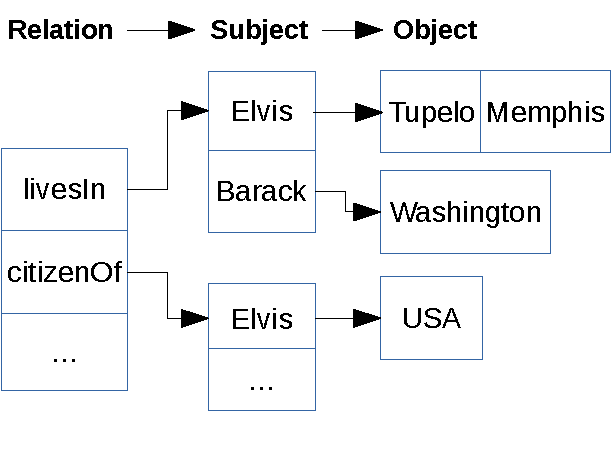
\includegraphics[width=0.5\textwidth]{figures/indexes}\
% \caption{Structure of the fact index RSO for a set of four facts}
% \label{indexes}
% \end{figure}
%
% In addition to the fact indexes, the database relies
% on three \emph{aggregated indexes} \texttt{S}, \texttt{P}, \texttt{O} that store the aggregated number of facts for each
% key of the fact indexes. For example, the aggregated index \texttt{P} stores the number of triples for each relation
% in the KB, e.g., $\{ livesIn=3, citizenOf=1 \}$ for the fact index depicted in Figure~\ref{indexes}.
% Fact indexes in combination with aggregated indexes can be used to efficiently fetch the instantiations of an atom.
% They also let us determine the size of atom, i.e., its number of bindings, in constant time.
% For example, the size of the atom $livesIn(x,y)$ can be retrieved by a simple look-up
% in the aggregated index \texttt{P}. In constrast, the size of the atom $livesIn(x, USA)$ requires two
% lookups in the fact index \texttt{ROS}: the first lookup to get the object values of $livesIn$ and the second
% to retrieve the list of subjects for the object value $USA$. If an atom has size greater than zero, it means
% that there exists a query answer for it in the KB.
%
% The existence of an answer for a conjunction of atoms in a KB is described in Algorithm~\ref{exists}.
% If the query contains a single atom (Line 3), we can directly verify if its size is greater than zero using
% the indexes (Line 4). Otherwise, we select the atom $B_s$ with fewest instantiations using the indexes (Line 6),
% and run through all of its instantiations (Lines 8 to 13). We apply such instantiations to the remaining atoms (Line 9)
% and repeate this process recursively (Line 10) until we end up with a single atom. Since rules are connected query patterns, the atom $B_s$ must share at least
% one variable with the remaining atoms. This means that by instantiating $B_s$, some variables in the remaining atoms
% become instantiated, making the atoms more selective with every recursive step.
%
% \begin{algorithm}
% \caption{Checking existence}
% \label{exists}
% \begin{algorithmic}[1]
% \Function{Exists}{$B_1 \wedge ... \wedge B_n$, $\mathcal{K}$}
%     \State $q := B_1 \wedge ... \wedge B_n$
%     \If {$length(q) = 1$}
%       \State \Return size($q$, $\mathcal{K}$) $> 0$
%     \Else
%       \State $B_s := findSmallest(q, \mathcal{K})$
%       \State $q := q - \{ B_s \} $
%       \ForAll {instantiations $b_s \in B_s$}
% 	\State Replace $b_s$ in $q$
% 	  \If{Exists($q$, $\mathcal{K}$)}
% 	    \State \Return true
% 	  \EndIf
%       \EndFor
%     \EndIf
%     \State \Return false
% \EndFunction
% \end{algorithmic}
% \end{algorithm}
%
% \paragraph{Implementation of Count-Projection Queries} Algorithm \ref{algi} shows how we answer count-projection queries
% of the form: \\ \\
% \noindent{SELECT $\bm{x}$, COUNT($H$) WHERE $H \wedge B_1 \wedge ... \wedge B_n$\\
% SUCH THAT COUNT($H$)$\geq k$} \\ \\
% These are the types of queries used to determine the relations and instances for new atoms in the specialization
% phase of AMIE. The algorithm takes as input a selection variable $\bm{x}$, a projection atom $H:=R(\bm{X},\bm{Y})$, remaining atoms $B_1, ... B_n$,
% and a KB $\mathcal{K}$.
% % For example, if the routine is used to find the relations for a new atom in a rule, e.g.,
% % $\bm{r}(\bm{Z}, \bm{W}) \wedge \vec{B} \Rightarrow r_h(x, y)$, then
% % $\bm{x} = \bm{r}$, $H = r_h(x, y)$ and $\bm{r}(\bm{Z}, \bm{W}) \wedge \vec{B}$ accounts for the set $B_1, ... B_n$.
% The algorithm returns a hash table with each instantiation of the selection variable
% $\bm{x}$ as key and the number of distinct bindings of the projection atom $H$ as value. Notice that Algorithm~\ref{algi}
% does not consider the threshold condition (SUCH THAT) since it is actually enforced by the AMIE algorithm and not
% the in-memory database.
%
% We first check whether $\bm{x}$ appears in the projection atom (Line 3).
% If that is the case (Lines 4 to 10), we run through all instantiations of the projection atom, instantiate the query accordingly (Line 6), and check for existence (Line 7).
% Each existing instantiation increases the counter for the respective value of the selection variable $\bm{x}$ (Line 8).
% If the selection variable does not appear in the projection atom (Lines 12 to 18),
% we iterate through all instantiations of the projection atom.
% We instantiate the query accordingly, and fire a SELECT query for $\bm{x}$ (Line 14).
% We then increase the counter for each value of $\bm{x}$ (Line 16).
%
% \paragraph{Implementation of Count Queries} Recall from Section~\ref{countQueries} that count queries in AMIE have the form \\ \\
% \noindent{SELECT COUNT($H'$) WHERE $H \wedge B_1 \wedge ... \wedge B_n$} \\
%
% These queries return the number of distinct bindings of the projection atom $H$
% that fullfill the pattern $H \wedge B_1 \wedge ... \wedge B_n$ and are used to
% calculate the confidence of rules. Since the aggregation function COUNT conveys
% distinct semantics, the in-memory database computes a SELECT DISTINCT query
% and then reports the size of the result set. Algorithm~\ref{select} describes
% the method to select the set of distinct bindings of the projection atom $H := r(\bm{X}, \bm{Y})$ in
% $H \wedge B_1 \wedge ... \wedge B_n$. Notice that this is not a general implementation of SELECT DISTINCT queries,
% since it is designed for binary atoms: it supports up to two variables that must occur in the same atom.
%
% Algorithm~\ref{select} starts finding the atoms with the fewest number of instantiations $B_s$. If such atom is the
% projection atom (Lines 5 to 11), i.e., $B_s = H$, the algorithm goes through all the instantiations $h$ of the $H$, instantiates
% the query accordingly and checks whether there exists a solution for the instantiated query pattern in the KB (Line 8).
% If it is the case, the solution $h$ is added to the result set. In contrast, if the most restrictive atom $B_s$ is not
% the projection atom (Lines 13 to 17), the algorithm iterates through the instantiations $b_s$ and recursively
% selects the solutions in the remaining atoms (Line 16).
%
% \begin{algorithm}
% \caption{Select distinct}
% \label{select}
% \begin{algorithmic}[1]
% \Function{Select}{$H$, $B_1 \wedge ... \wedge B_n$, $\mathcal{K}$}
%     \State $q := H \wedge B_1 \wedge ... \wedge B_n$
%     \State $B_s := findSmallest(q)$
%     \State $result := [ ]$
%     \If{$B_s = H$}
%       \ForAll instantiations $h \in H$
% 	\State Replace $h$ in $q$
% 	\If {Exists($q$, $\mathcal{K}$)}
% 	  \State $result$.add($h$)
% 	\EndIf
%       \EndFor
%     \Else
%       \State $q := q - \{ B_s\}$
%       \ForAll{instantiations $b_s \in B_s$}
%       	\State Replace $b_s$ in $q$
%       	\State $result$.add(Select($H$, $q$, $\mathcal{K}$))
%       \EndFor
%     \EndIf
%     \State \Return $result$
% \EndFunction
% \end{algorithmic}
% \end{algorithm}
%
% \paragraph{Summary}
% The AMIE algorithm iteratively builds more complex rules from simpler rules by the help of three operators.
% It takes advantage of monotonic measures to prune the search space efficiently and also takes care of duplicate elimination.
% We have identified projection queries as the crucial type of queries for rule mining.
% Since standard database systems and standard SPARQL systems provide no specifically tuned support for these queries,
% we have implemented a vanilla in-memory database, which has specific support for projection queries.
% Our entire implementation is in Java. The code can be downloaded from our Web site\footnote{\url{http://mpi-inf.mpg.de/departments/ontologies/projects/amie}}.
%
%
% \begin{algorithm}
% \caption{Answering Projection Queries}
% \label{algi}
% \begin{algorithmic}[1]
% \Function{SELECT}{$\bm{x}$, $R(X,Y) \wedge B_1 \wedge ... \wedge B_n$, $\mathcal{K}$}
%     \State $map = \{\}$
%     \State $q=B_1 \wedge ... \wedge B_n$
%     \If {$\bm{x} \in \{R,X,Y\}$}
% 	  \ForAll{instantiations $r(x,y) \in R(\bm{X}, \bm{Y})$}
% 	    \State In $q$, replace $R$ by $r$, $X$ by $x$, $Y$ by $y$
% 	    \If{Exists($q$, $\mathcal{K}$)}
% 		\State $map[x]++$
% 	    \EndIf
% 	  \EndFor
% 	\Else
% 	  \ForAll{instantiations $r(x,y) \in R(\bm{X},\bm{Y})$}
% 	    \State In $q$, replace $R$ by $r$, $X$ by $x$, $Y$ by $y$
% 	    \State $\mathcal{X} :=$ SELECT DISTINCT $\bm{x}$ FROM $\mathcal{K}$ WHERE $q$
% 	    \ForAll{$x \in \mathcal{X}$}
% 		  \State $map[x]++$
% 	    \EndFor
% 	  \EndFor
% 	\EndIf
% 	\State \Return $map$
% \EndFunction
% \end{algorithmic}
% \end{algorithm}
% \ \\[-1cm]
% }